\documentclass[space]{ctexart} % ans
\usepackage{ZSuniv}
\usepackage{tikz}
\usepackage{fancybox}
\usepackage{enumitem}
\usetikzlibrary{patterns}
\topskip=1.5cm

\newcommand*\circled[1]{\raisebox{.5pt}{\textcircled{\raisebox{-.4pt} {\fontsize{12pt}{16pt}\selectfont#1}}}}
\newcommand*\circledt[2]{\raisebox{.5pt}{\textcircled{\raisebox{-.4pt} {{\fontsize{9pt}{15pt}\selectfont#1\hspace*{-0.25mm}#2}}}}}
\def\ge{\geqslant}
\def\geq{\geqslant}
\def\le{\leqslant}
\def\leq{\leqslant}

\newcommand*\emptycirc[1][1ex]{\tikz\draw[line width=2pt] (0,0) circle (#1);}

\begin{document}\zihao{4}
% _______________________________________
% ***************************************
\fancypage{
\setlength{\fboxsep}{8pt}%
\setlength{\fboxrule}{1.5pt}%
\setlength{\shadowsize}{0pt}%
\shadowbox}{}
% =======================================

%%2009
%% _______________________________________
%% ***************************************
%\univ{~}
%\biaoti{二\,\raisebox{-.5ex}{\emptycirc{~}}\!\raisebox{-.5ex}{\emptycirc{~}}\!九年招收攻读硕士学位研究生入学考试试题}
%\DMKM
%\tishi{(答案必须写在答题纸上, 写在试题上无效)}
%
%\vspace*{0.5cm}
%\begin{enumerate}[itemsep=1.2em,label=\arabic*.,topsep=0pt,left=0em]
%\item 计算题. (每小题6分, 共48分)
%
%
%\setcounter{enumii}{0}
%\begin{enumerate}[itemsep=1.2em,label=(\arabic*),topsep=0pt,left=2em] % itemsep 参数是两个 item 内容之间的间距
%	\item 求
%\begin{align*}
%\lim\limits_{x \rightarrow \infty}\left(x-x^{2} \ln \left(1+\frac{1}{x}\right)\right).
%\end{align*}
%
%    \item $\begin{cases}
%x=\cos \left(t^{2}\right) \\
%y=\displaystyle{\int_{0}^{2}} \dfrac{\sin u}{u} {\rm d} u
%\end{cases}$, 求 $\dfrac{{\rm d} y}{{\rm d}x}$.
%
%
%   \item 求
%\begin{align*}
%\int \dfrac{1-\ln x}{\ln ^{2} x} {\rm d} x.
%\end{align*}
%
%    \item 求
%\begin{align*}
%\int_{-1}^{1}|x-a| {\rm e}^{x} {\rm d} x,|a|<1.
%\end{align*}
%
%
%    \item 设$z=u v+\sin t, u=e^{t}, v=\cos t$, 求$\dfrac{{\rm d} z}{{\rm d} t}$.
%
%    \item 设$u=\varphi(x+\psi(y))$, 其中$\varphi, \psi$ 二阶可导, $x, y$ 为自变量, 求${\rm d}^{2} u$.
%
%    \item 求级数
%    \begin{align*}
%      \sum\limits_{n=1}^{\infty} \cos^n x
%    \end{align*}
%    在收敛域上的和函数.
%
%    \item 判别级数
%    \begin{align*}
%      \sum\limits_{n=1}^{\infty} \dfrac{1}{n^{1+\dfrac{1}{n}}}
%    \end{align*}
%    的收敛性.
%
%\end{enumerate}
%
%\item (12分) 将区间$[1,2]$作$n$等分, 等分点为$1=x_0<x_1<x_2<\ldots<x_n=2$, 求
%\begin{align*}
%\lim\limits_{n\rightarrow \infty}\sqrt[n]{x_1x_2x_3\ldots x_n}.
%\end{align*}
%
%\item (16分) 计算
%\begin{align*}
%    \iint\limits_{\Sigma} x^{2} {\rm d} y {\rm d} z+y^{2} {\rm d} z {\rm d} x+z^{2} {\rm d} x {\rm d} y
%\end{align*}
%其中  $\ell$  是从点  $A(-1,0)$  到点  $B(1,0)$  的一条不通过原点的光滑曲线:  $y=f(x)$, $x \in[-1,1]$, 且当  $x \in(-1,1)$  时,  $f(x)>0 $.
%
%\item (16分) 计算
%\begin{align*}
%    \iint\limits_{\Sigma} x^{2} \mathrm{~d} y \mathrm{~d} z+y^{2} \mathrm{~d} z \mathrm{~d} x+z^{2} \mathrm{~d} x \mathrm{~d} y
%\end{align*}
%其中  $\Sigma $ 为曲面 $ x^{2}+y^{2}=z^{2}$  介于平面  $z=0$  和  $z=h(h>0)$  之间的部分取下侧.
%
%\item (16分) 设 $ f(x)$  在 $ [1, \infty)$  连续,  $f^{\prime \prime}(x) \leq 0$, $f(1)=2$, $f^{\prime}(1)=-3 $.  证明:  $f(x)=0 $ 在  $(1, \infty)$  有且仅有一个实根.
%
%\item (16分) 设函数 $f(x) $ 在 $(-\infty, \infty)$ 连续, 试证: 对一切 $x$ 满足 $f(2 x)=f(x) e^{x}$ 的充要条件是 $f(x)=f(0) e^{x} $.
%
%\item (16分) 求椭球面
%\begin{align*}
%    \frac{x^{2}}{a^{2}}+\frac{y^{2}}{b^{2}}+\frac{z^{2}}{c^{2}}=1
%\end{align*}
%在第一象限部分的切平面与三坐标平面围城的四面体的最小体积.
%
%\item (10分) 讨论
%\begin{align*}
%    \frac{x^{2}}{a^{2}}+\frac{y^{2}}{b^{2}}+\frac{z^{2}}{c^{2}}=1
%\end{align*}
%的收敛性.
%
%\end{enumerate}
%
%\clearpage	
%	
%2010
% _______________________________________
% ***************************************
\univ{~}
\biaoti{二\,\raisebox{-.5ex}{\emptycirc{~}}\!一\,\raisebox{-.5ex}{\emptycirc{~}}\!年招收攻读硕士学位研究生入学考试试题}
\DMKM
\tishi{(答案必须写在答题纸上, 写在试题上无效)}

\vspace*{0.5cm}
\begin{enumerate}[itemsep=1.5em,label=\arabic*.,topsep=0pt,left=0em]
\item 计算题. (每小题6分, 共48分)


\setcounter{enumii}{0}
\begin{enumerate}[itemsep=1em,label=(\arabic*),topsep=0pt,left=2em] % itemsep 参数是两个 item 内容之间的间距
	\item 求极限
\begin{align*}
\lim\limits_{n \rightarrow \infty} \frac{1}{n} \sqrt[n]{n(n+1) \cdots(2 n+1)}.
\end{align*}

    \item 计算不定积分
    \begin{align*}
      \int \max (|x|, 1) {\rm d} x.
    \end{align*}


   \item 已知$f(x)=\displaystyle{\int_{0}^{x}} \frac{\sin t}{\pi-t} \mathrm{~d} t$, 求不定积分
   \begin{align*}
   \int_{0}^{\pi} f(x) \mathrm{d} x
   \end{align*}

    \item 求二元函数极限
\begin{align*}
\lim\limits_{x \rightarrow 0, y \rightarrow 0}\left(x^{2}+y^{2}\right)^{x^{2} y^{2}}.
\end{align*}

  \item 求二次积分
  \begin{align*}
  \int_{0}^{1} \mathrm{~d} y \int_{y}^{1} e^{x^{2}} \mathrm{~d} x
  \end{align*}

  \item 计算
  \begin{align*}
  I=\oint_{L} \frac{x \mathrm{~d} y-y \mathrm{~d} x}{x^{2}+y^{2}}
  \end{align*}
其中  $L$ 为一条无重点, 分段光滑且不经过原点的连续封闭曲线, $L$ 的方向为逆时针方向.

\item 讨论数项级数
  \begin{align*}
 \sum_{n=1}^{\infty} \frac{(1-\cos x) \sin n x}{\sqrt{n+x}}
  \end{align*}
在  $[0,2\pi]$ 上的一致收敛性.

\item 计算
  \begin{align*}
 \iint_{s}\left(x^{2}+y^{2}\right) \mathrm{d} S.
  \end{align*}
其中 $S$ 为曲面  $z=\sqrt{x^{2}+y^{2}}$ 与平面 $z=1$ 所围几何体的表面.

\end{enumerate}



\item (12分) 单位圆盘中切去圆心角为  $\theta$  的扇形, 余下部分粘合成一雉面. 问  $\theta$ 为多少时, 该雉面加上底面所围成
的雉体体积最大?

\item (16分) 设 f(x) 在 $x=0$ 某邻域内有二阶连续导数, 且 $\lim\limits_{x \rightarrow 0} \dfrac{f(x)}{x}=0$.  证明:
\begin{align*}
    \sum_{n=1}^{\infty} f\left(\frac{1}{n}\right)
\end{align*}
绝对收敛.

\item (16分) 设
\begin{align*}
    f(x, y)=\begin{cases}
\left(x^{2}+y^{2}\right)^{p} \sin \frac{1}{x^{2}+y^{2}}, & x^{2}+y^{2} \neq 0 \\
0, & x^{2}+y^{2}=0
\end{cases}
\end{align*}
其中  $p$ 为正数. 试分别确定 $p$ 的值, 使得如下结论分别成立:
\begin{enumerate}[itemsep=0em,label=(\arabic*),topsep=0pt,left=0em]
\item  $f(x, y)$  在点  $(0,0)$  处连续;
\item   $f_{x}(0,0)$  与  $f_{y}(0,0)$  都存在;
\item   $f_{x}(x, y)$  与  $f_{y}(x, y)$  在  $(0,0)$  点连续.
\end{enumerate}

\item (16分) 计算由曲面
\begin{align*}
    \left(\frac{x}{a}+\frac{y}{b}\right)^{2}+\left(\frac{z}{c}\right)^{2}=1,(x \geq 0, y \geq 0, z \geq 0, a>0, b>0, c>0)
\end{align*}
所围成几何体的体积 , 其中 $a,b,c$ 为正常数.

\item (16分) 讨论
\begin{align*}
    \sum_{n=1}^{\infty} \frac{n^{2}+1}{n ! 2^{n}} x^{n}
\end{align*}
的收敛范围, 并求其和函数.


\item (16分)  设 $ u=f(r)$, 其中  $r=\sqrt{x^{2}+y^{2}+z^{2}}$. 变换方程:  $\frac{\partial^{2} u}{\partial x^{2}}+\frac{\partial^{2} u}{\partial y^{2}}+\frac{\partial^{2} u}{\partial z^{2}}=0$, 使其成为关于  $f(r)$ 的方程.

\newpage
\item (10分) 判别级数
\begin{align*}
   \sqrt{2}+\sqrt{2-\sqrt{2}}+\sqrt{2-\sqrt{2+\sqrt{2}}}+\sqrt{2-\sqrt{2+\sqrt{2+\sqrt{2}}}}+\cdots
\end{align*}
的收敛性.


\end{enumerate}

\clearpage	

%2011
% _______________________________________
% ***************************************
\univ{~}
\biaoti{二\,\raisebox{-.5ex}{\emptycirc{~}}\!一一年招收攻读硕士学位研究生入学考试试题}
\DMKM
\tishi{(答案必须写在答题纸上, 写在试题上无效)}

\vspace*{0.5cm}
\begin{enumerate}[itemsep=1.5em,label=\arabic*.,topsep=0pt,left=0em]
\item 计算题. (每小题6分, 共48分)


\setcounter{enumii}{0}
\begin{enumerate}[itemsep=1em,label=(\arabic*),topsep=0pt,left=2em] % itemsep 参数是两个 item 内容之间的间距
	\item 求极限
\begin{align*}
\lim\limits_{x \rightarrow 0} \frac{\sqrt{1-x^{2}}-1}{x \tan x}.
\end{align*}

    \item 计算积分
    \begin{align*}
     \int_{0}^{\frac{\pi}{2}} \frac{\sin x \cos x}{1+\sin ^{4} x} \mathrm{~d} x
    \end{align*}


   \item 已知  $\sum_{n=1}^{\infty}(-1)^{n} a_{n}=A$, $\sum_{n=1}^{\infty} a_{2 n-1}=B$, 求级数 $\sum_{n=1}^{\infty} a_{n}$ 的和.

    \item 计算
\begin{align*}
\iint\limits_{\Omega}\left(2x+\frac{4}{3}y+z\right){\rm d}S.
\end{align*}
其中 $\Omega$ 为平面 $\frac{x}{2}+\frac{y}{3}+\frac{z}{4}=1$ 在第一象限的部分.


\item 计算
  \begin{align*}
  \int\nolimits_{L}\sqrt{x^2+y^x}{\rm d}x+y\left(xy+\ln\left(x+\sqrt{x^2+y^2}\right)\right){\rm d}y
  \end{align*}
其中  $L$ 为曲线 $y=\sin x (0\leq x \leq \pi)$ 按 $x$ 增大方向.

  \item 判别级数
  \begin{align*}
  \sum_{n=1}^{\infty}{\frac{(-1)^n}{\sqrt{n}-\ln n}}
  \end{align*}
是绝对收敛, 条件收敛, 还是发散?


\item 设$\begin{cases}
          x=t^3-3t\\
          y=t^2-2t\\
        \end{cases}$,
求二阶导数 $\dfrac{{\rm d}^2 y}{{\rm d}x^2}$.

\item 求极限
\begin{align*}
  \lim\limits_{n\rightarrow \infty}\frac{1}{2}\cdot\frac{3}{4}\cdot\cdots\cdot\frac{2n-1}{2n}.
\end{align*}

\end{enumerate}



\item (12分) 设
\begin{align*}
  f(x,y)\sqrt{|xy|}.
\end{align*}
求偏导数 $\dfrac{\partial f}{\partial x}$, $\dfrac{\partial f}{\partial y}$, 并讨论 $f(x,y)$ 在点 $(0,0)$ 处的可微性.


\item (16 分) 设 $f(x)$ 满足:\\
 \circled{1} $-\infty<a\leq f(x) \leq b<+\infty$;\\
 \circled{2} $|f(x)-f(y)| \leq L|x-y|$, $0<L<1$, $x, y \in[a, b]$;\\
任取  $x_{1} \in[a, b]$, 作序列 $x_{n+1}=\frac{1}{2}\left(x_{n}+f\left(x_{n}\right)\right)$, $n=1,2, \cdots$. 求证: $\left\{x_{n}\right\}$  收敛, 且其极限  $\xi \in[a, b]$  满足:
$f(\xi)=\xi$.


\item (16分) 设正项级数列 $\{a_{n}\}$ 单调递增, 且 $\lim\limits_{n\rightarrow \infty}=+\infty$.
\begin{align*}
    \sum_{n=1}^{\infty} \left(1-\frac{x_{n}}{x_{n+1}}\right)
\end{align*}
发散.

\item (16分) 已知  $P$  是  $\angle A O B $ 内一固定点,  $\angle A O P=\alpha$, $\angle B O P=\beta $, 线段长度 $ \overline{OP}=L $, 过  $P$  的直线交射线  $O A$  和 $ O B $ 于点 $ X$  和 $ Y $. 求线段长度乘积 $ \overline{P X} \cdot \overline{P Y}$  的最小值, 说明取最值时  $X, Y $ 的位置.

\item (16分) 计算由曲面积分
\begin{align*}
    I=\iint\limits_{\Omega}4z{\rm d}y{\rm d}z-2zy{\rm d}z{\rm d}x+
    (1-z^2){\rm d}x{\rm d}y.
\end{align*}
 其中  $\Omega$ 是由曲线 $\begin{cases}
     z=e^{y} \\
    x=0
 \end{cases},(0 \leq y \leq a)$ 绕 $z $轴旋转一周所成曲面的下侧.

 \item (16分)  设  $f_{1}(x)=f(x)=\frac{x}{\sqrt{1+x^{2}}}$, $f_{n+1}(x)=f\left(f_{n}(x)\right)$, $n=1,2, \cdots $.  证明: 函数项级数
\begin{align*}
    f_{1}(x)+\sum_{n=1}^{\infty}\left(f_{n+1}(x)-f_{n}(x)\right)
\end{align*}
 在  $(-\infty,+\infty)$  上一致收敛于零.

 \newpage
 \item  (10 分)  设 $ 0<x<1 $, 求
 \begin{align*}
     \sum_{n=0}^{\infty} \frac{x^{2^{n}}}{1-x^{2^{n+1}}}
 \end{align*}
 的和函数.

\end{enumerate}

\clearpage	


%2012
% _______________________________________
% ***************************************
\univ{~}
\biaoti{二\,\raisebox{-.5ex}{\emptycirc{~}}\!一二年招收攻读硕士学位研究生入学考试试题}
\DMKM
\tishi{(答案必须写在答题纸上, 写在试题上无效)}

\vspace*{0.5cm}
\begin{enumerate}[itemsep=1.2em,label=\arabic*.,topsep=0pt,left=0em]
\item 计算题. (每小题6分, 共48分)

\setcounter{enumii}{0}
\begin{enumerate}[itemsep=1.2em,label=(\arabic*),topsep=0pt,left=2em] % itemsep 参数是两个 item 内容之间的间距

\item  求极限
\begin{align*}
\lim\limits_{x \rightarrow 0}\left(1+x^{2} e^{x}\right)^{\frac{1}{1-\cos x}}
\end{align*}


\item   给定  $a_{0}, a_{1} $, 并设 $ a_{n}=\frac{1}{2}\left(a_{n-1}+a_{n-2}\right)$, $n \geq 2 $, 求:  $\lim\limits_{n \rightarrow \infty} a_{n} $.

\item 求
\begin{align*}
I_{n}=\int_{0}^{n \pi} x|\sin x| \mathrm{d} x.
\end{align*}

\item  设  $g(x), f(x, y)$  均二阶可微, $ u(x, y)=y g(\cos x)+f\left(e^{x}, x y\right) $, 求 $ \frac{\partial u}{\partial x}$, $\frac{\partial^{2} u}{\partial x \partial y} $.

\item 已知二粗圆抛物面为 $ \Sigma_{1}: z=x^{2}+2 y^{2}+1$, $\Sigma_{2}: z=2\left(x^{2}+3 y^{2}\right) $, 计算 $ \Sigma_{1} $ 被  $\Sigma_{2} $ 截下部分的曲面面积.

\item  求曲线积分
\begin{align*}
\oint_{C} \frac{(x+4 y) \mathrm{d} y+(x-y) \mathrm{d} x}{x^{2}+4 y^{2}} .
\end{align*}
其中 $ C $ 为以原点为圆心单位圆, 并取正向.

\item  判断级数
\begin{align*}
\sum_{n=1}^{\infty} n !\left(\frac{-e}{n}\right)^{n}
\end{align*}
的玫散性.

\item  设  $a_{n}>0$, $\lim\limits_{n \rightarrow \infty} a_{n}=a>0 $, 讨论级数
\begin{align*}
\sum_{n=1}^{\infty}\left(\frac{a}{a_{n}}\right)^{n}
\end{align*}
的玫散性.

\end{enumerate}

\item (16 分)  给出函数 $ f(x)=x\left[x^{-1}\right] $ 在 $ (0,+\infty) $ 上的不连续点, 其中 $ \left[x^{-1}\right] $ 表示 $ x^{-1} $ 的整数部分.

\item  (16分) 设
\begin{align*}
f(x, y)=\begin{cases}
    \frac{x^{\alpha} y}{x^{2}+y^{2}}, & (x, y) \neq(0,0) \\
0, & (x, y)=(0,0)
\end{cases}.
\end{align*}
问  $\alpha $ 取何值时能使 $ f(x, y) $ 在点 $ (0,0) $ 可微?

\item (16 分)  计算曲线积分
\begin{align*}
\oint_{L}(y+1) \mathrm{d} x+(z+2) \mathrm{d} y+(x+3) \mathrm{d} z
\end{align*}
其中 $ L $ 是球面 $ x^{2}+y^{2}+z^{2}=R^{2}$  被平面 $ x+y+z=0 $ 所截得的圆周, 从 $ x $ 轴正向看去, $ L$ 是逆时针方向.

\item  (16分)  讨论函数项级数
\begin{align*}
\sum_{n=1}^{\infty} \frac{x^{n}}{n \ln n}
\end{align*}
在  $[0,1) $ 上的一致收敛性.

\item  (16分)  设  $f(x)$  在  $[a, b] $ 上有二阶连续导数, $ f\left(\frac{a+b}{2}\right)=0 $, 求证:
\begin{align*}
\left|\int_{a}^{b} f(x) \mathrm{d} x\right| \leq \frac{(b-a)^{3}}{24} \max _{a \leq x \leq b}\left|f^{\prime \prime}(x)\right| .
\end{align*}

\item   (10分) 证明不等式
\begin{align*}
y x^{y}(1-x)<e^{-1}
\end{align*}
其中 $ (x, y) \in D=\{(x, y) \mid 0<x<1, y>0\} $.

\item  (12 分) 设 $ x>a $ 时 $ g(x)>0$, $f(x) $ 和 $ g(x) $ 在任意有限区间 $ [a, b] $ 上可积, $ \int_{a}^{+\infty} g(x) \mathrm{d} x $ 发散, 且 $ \lim\limits_{x \rightarrow+\infty} \frac{f(x)}{g(x)}=
0$, 证明:
\begin{align*}
\lim\limits_{x \rightarrow+\infty} \frac{\int_{a}^{x} f(x) \mathrm{d} x}{\int_{a}^{x} g(x) \mathrm{d} x}=0
\end{align*}


\end{enumerate}

\clearpage	

%2013
% _______________________________________
% ***************************************
\univ{~}
\biaoti{二\,\raisebox{-.5ex}{\emptycirc{~}}\!一三年招收攻读硕士学位研究生入学考试试题}
\DMKM
\tishi{(答案必须写在答题纸上, 写在试题上无效)}

\vspace*{0.5cm}
\begin{enumerate}[itemsep=1.2em,label=\arabic*.,topsep=0pt,left=0em]
\item 计算题. (每小题8分, 共24分)


\setcounter{enumii}{0}
\begin{enumerate}[itemsep=1.2em,label=(\arabic*),topsep=0pt,left=2em] % itemsep 参数是两个 item 内容之间的间距

\item  设
\begin{align*}
x_{n}=\sqrt[n]{\left[1+\left(\frac{1}{n}\right)^{2}\right]\left[1+\left(\frac{2}{n}\right)^{2}\right] \cdots\left[1+\left(\frac{n}{n}\right)^{2}\right]}
\end{align*}
 求  $\lim\limits_{n \rightarrow \infty} x_{n}$.

 \item $\lim\limits_{n \rightarrow \infty} n^{2}\left(x^{\frac{1}{n}}-x^{\frac{1}{n+1}}\right) $, 其中 $ x>0 $.

 \item  $\lim\limits_{m \rightarrow \infty} \frac{\left(\sum_{i=d}^{m} i^{d}\right)-\frac{m^{d+1}}{d+1}}{m^{d}} $, 其中 $ d>0 $.

\end{enumerate}

\item  (20分)(1)  叙述数列 $ \left\{a_{n}\right\} $ 收敛的柯西收敛准则并证明之.\\
(2) 用柯西收敘准则证明: 数列 $ a_{n}=\frac{1}{2 \ln 2}+\frac{1}{3 \ln 3}+\cdots+\frac{1}{n \ln n} $ 趋于无穷大.
\item  (20分)  证明:\\
(1)  $f(x)=\sin \sqrt{x} $ 在 $ [0, \infty) $ 上一致连续.\\
(2) $ g(x)=\sin x^{2} $ 在 $ [0, \infty) $ 上不一致连续.

\item  (16 分)  设 $ x_{1}=-1$, $x_{n+1}=-1+\frac{x_{n}^{2}}{2}(n=1,2, \cdots) $, 证明  $\lim\limits_{n \rightarrow \infty} x_{n} $ 存在.

\item  ( 10 分) 设 $ a_{n}>0, n=1,2, \cdots $, 证明
\begin{align*}
\varlimsup_{n \rightarrow \infty} n\left(\frac{1+a_{n+1}}{a_{n}}-1\right) \geq 1 .
\end{align*}

\item (10分)  设 $ 0<x<1 $, 求
\begin{align*}
S(x)=\sum_{k=1}^{\infty} x^{k}(1-x)^{2 k}
\end{align*}
的极值.


\item (10 分)  计算
\begin{align*}
\int_{C} \frac{(x+y) \mathrm{d} x-(x-y) \mathrm{d} y}{x^{2}+y^{2}}
\end{align*}
其中 $ C $ 是一条从 $ (-1,0) $ 到 $ (1,0) $ 不经过原点的光滑曲线:  $y=f(x),-1 \leq x \leq 1 $.

\item ( 12分) 计算
\begin{align*}
\iint_{S} y z \mathrm{~d} x \mathrm{~d} y+z x \mathrm{~d} y \mathrm{~d} z+x y \mathrm{~d} z \mathrm{~d} x
\end{align*}
其中 $ S $ 是由 $ x^{2}+y^{2}=1 $, 三个坐标平面及 $ z=2-x^{2}-y^{2}$  所围立体图形在第一卦限的外侧.

\item  (12 分)  讨论级数
\begin{align*}
\sum_{k=1}^{\infty} \frac{\sin k x}{k}
\end{align*}
在 $ [0,2 \pi] $ 上的一致收敛性.

\item  (16 分 )(1)  分别将函数 $ f(x)=\frac{\pi-x}{2}$  和  $g(x)=
\begin{cases}
  (\pi-1) x, &0 \leq x \leq 1 \\
  \pi-x, &1<x \leq \pi
\end{cases}$
在 $ [0, \pi] $ 按正弦 Fourier 级数展开.\\
(2) 证明: $ \sum_{n=1}^{\infty} \frac{\sin n}{n}=\sum_{n=1}^{\infty}\left(\frac{\sin n}{n}\right)^{2} $.

\end{enumerate}

\clearpage	

% 2014
% _______________________________________
% ***************************************
\univ{~}
\biaoti{二\,\raisebox{-.5ex}{\emptycirc{~}}\!一四年招收攻读硕士学位研究生入学考试试题}
\DMKM
\tishi{(答案必须写在答题纸上, 写在试题上无效)}

\vspace*{0.5cm}
\begin{enumerate}[itemsep=1.2em,label=\arabic*.,topsep=0pt,left=0em]
\item ( 30 分)计算

\setcounter{enumii}{0}
\begin{enumerate}[itemsep=1.2em,label=(\arabic*),topsep=0pt,left=2em] % itemsep 参数是两个 item 内容之间的间距

  \item $\int \frac{1}{x} \sqrt{\frac{x+2}{x-2}} \mathrm{~d} x $.

  \item  $\int_{\Gamma} x y \mathrm{~d} s $, 其中  $\Gamma $ 为 $ x^{2}+y^{2}+z^{2}=a^{2} $ 与 $ x+y+z=0 $ 的交线.

  \item  $\lim _{n \rightarrow \infty}\left(\int_{0}^{\pi} x^{2013} \sin ^{n} x \mathrm{~d} x\right)^{\frac{1}{n}}$.

\end{enumerate}

\item   (10分) 设 $ f(x) $ 在 $ (-\infty,+\infty) $ 上连续, 并且  $\int_{-\infty}^{+\infty} f(x) \mathrm{d} x $ 收敛, 对任意 $ a, b, c \in \mathbb{R}$  都有 $ \int_{a}^{a+c} f(x) \mathrm{d} x=
 \int_{b}^{b+c} f(x) \mathrm{d} x $ 证明: $ f(x) \equiv 0 $.

\item   ( 15 分) 表格填空:\\
\begin{center}
\begin{tabular}{|c|l|l|l|}
\hline $\sum_{n=3}^{\infty} a^{n} n^{b}(\ln n)^{c} $ & 绝对收敛 & 条件收敛 & 发散 \\
\hline 参数 $ a, b, c$  的取值范围 & & & \\
\hline
\end{tabular}
\end{center}

\item   (10 分)  求方程组
\begin{align*}
\begin{cases}
    u+v=x+y \\
\frac{\sin u}{\sin v}=\frac{x}{y}
\end{cases}
\end{align*}
所确定的隐函数 $ \begin{cases}
    u=u(x, y) \\
     v=v(x, y)
\end{cases}$
 的微分  $\mathrm{d} u, \mathrm{~d} v $.

\item (10 分)  讨论函数
\begin{align*}
\int_{0}^{\infty} \sin x^{2} \mathrm{~d} x; \int_{0}^{\infty} \int_{0}^{\infty} \sin \left(x^{2}+y^{2}\right) \mathrm{d} x \mathrm{~d} y
\end{align*}
的敛散性. 其中 $ \int_{0}^{\infty} \int_{0}^{\infty} \sin \left(x^{2}+y^{2}\right) \mathrm{d} x \mathrm{~d} y=\lim _{r \rightarrow \infty \atop x^{2}+y^{2} \leq r^{2} ; x, y \geq 0} \sin \left(x^{2}+y^{2}\right) \mathrm{d} x \mathrm{~d} y $.

\item (10 分)  讨论广义积分
\begin{align*}
    f(x, y)=\begin{cases}
    x^{\frac{3}{2}} \sin \frac{y}{x}, & x \neq 0 \\
        0, & x=0
    \end{cases}
\end{align*}
的可微性.

\item (15 分)  讨论积分
\begin{align*}
    f(x)=\int_{0}^{\infty} e^{-x\left(t+\frac{1}{t}\right)} \mathrm{d} t
\end{align*}
的收敛域和$f(x)$的连续性.

\item (10 分) 半径为 $ r $ 的球的中心在单位球 $ x^{2}+y^{2}+z^{2}=1 $ 的表面上, 问 $ r $ 取何值时该球位于单位球内部分的表 面积最大?

\item (15分) 设$  a>0 $, 求 $ y^{2}=\frac{x^{3}}{2 a-x}  $与 $ x=2 a$  所围成的面积.

\item ( 15 分  )  讨论
\begin{align*}
f(x)=x \sin x
\end{align*}
在 $ [1, \infty)$  上是否一致连续, 并说明理由.

\item ( 15 分)  设 $ f(x)=\int_{x}^{x^{2}}\left(1+\frac{1}{2 t}\right)^{t}\left(e^{\frac{1}{\sqrt{t}}}-1\right) \mathrm{d} t,(x>0) $.  求
\begin{align*}
\lim\limits_{n \rightarrow \infty} f(n) \sin \frac{1}{n}
\end{align*}


\end{enumerate}

\clearpage	

%2015
% _______________________________________
% ***************************************
\univ{~}
\biaoti{二\,\raisebox{-.5ex}{\emptycirc{~}}\!一五年招收攻读硕士学位研究生入学考试试题}
\DMKM
\tishi{(答案必须写在答题纸上, 写在试题上无效)}

\vspace*{0.5cm}
\begin{enumerate}[itemsep=1.2em,label=\arabic*.,topsep=0pt,left=0em]
\item 计算题. (每小题15分, 共60分)

\setcounter{enumii}{0}
\begin{enumerate}[itemsep=1.2em,label=(\arabic*),topsep=0pt,left=2em]
	\item 求极限
\begin{align*}
    \lim _{x \rightarrow 0}\left(\frac{\sin x}{x}\right)^{\frac{1}{1-\cos x}}.
\end{align*}

    \item 已知  $y=e^{x} \cdot x^{\sin x} $, 求 $ \frac{\mathrm{d} y}{\mathrm{~d} x} $.

    \item 设  $f(x, y, z)=x y^{2} z^{3} $, 且 $z=z(x, y) $ 是由方程 $ x^{2}+y^{2}+z^{2}-3 x y z=0 $ 所确定的隐函数, 求 $ f_{x}(1,1,1) $.

    \item 求 $ u=x-2 y+2 z $ 在条件 $ x^{2}+y^{2}+z^{2}=1 $ 下的条件极值(含极大值和极小值) .

\end{enumerate}

\item ( 15 分)  将 $ \frac{1}{x^{2}+4 x+3} $ 展开为$  x-1 $ 的幕级数.

\item (15 分)  求抛物面
\begin{align*}
z=x^{2}+y^{2}
\end{align*}
与抛物柱面
\begin{align*}
y=x^{2}
\end{align*}
的交线上的点 $ P(1,1,2) $ 处的切线方程和平面方程.

\item  (15分)  计算三重积分
\begin{align*}
\iiint_{\Omega}(x+y+z) \mathrm{d} x \mathrm{~d} y \mathrm{~d} z
\end{align*}
其中 $ \Omega $ 是由平面$  x+y+z=1 $ 与三个坐标面围成的区域.


\item (20 分)  如下图所示, 设当  $0 \leq x \leq a $ 时, 直线  $y=a x(0<a<1)$  与抛物线  $y=x^{2} $ 所围成的图形面积为 $ S_{1}$ . 当 $ a \leq x \leq 1 $ 时, 直线 $ y=a x(0<a<1) $, 拖物线 $ y=x^{2} $ 与直线 $ x=1 $ 所围成的图形的面积为 $ S_{2}$

\begin{center}
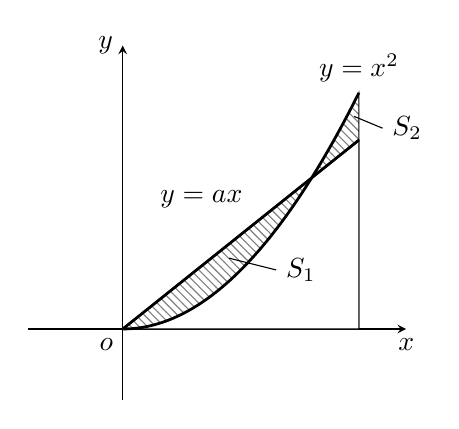
\begin{tikzpicture}[scale=3]
\draw[-stealth] (-0.4,0)--(1.2,0) node[below,scale=1]{$x$};
\draw[-stealth] (0,-0.3)--(0,1.2) node[left,scale=1]{$y$};
\draw (0,0) node [below left,scale=1] {$o$};
\filldraw [pattern=north west lines,pattern color=gray] (0,0) -- plot [domain=0:1,smooth] (\x,{\x*\x}) --   (1,0) -- (0,0);
\filldraw [fill=white] (0,0) -- plot [domain=0:1,smooth] (\x,{0.8*\x}) --   (1,0) -- (0,0);
\filldraw [pattern=north west lines,pattern color=gray] (0,0) -- plot [domain=0:0.8,smooth] (\x,{0.8*\x}) --  plot [domain=0:0.8,smooth] (\x,{\x*\x}) -- (0,0);
\draw[domain=0:1,smooth,line width=1pt] plot (\x,{\x*\x}) node[above] {$y=x^2$};
\draw[domain=0:1,smooth,line width=1pt] plot (\x,{0.8*\x})node[left=2cm,above=-1cm]{$y=ax$};
\draw (0.45,0.3)--(0.65,0.25)node[right]{$S_{1}$};
\draw (0.98,0.9)--(1.1,0.85)node[right]{$S_{2}$};
\end{tikzpicture}
\end{center}

(1) 确定 $ a $ 的值, 使 $ S=S_{1}+S_{2} $ 达到最小, 并求出最小值.

(2) 求当 $ S=S_{1}+S_{2} $ 达到最小值时, 该图形绕 $ x $ 轴旋转一周所得到的旋转体的体积.


6. (25分)  设 $ f(x) $ 在 $ (-\infty,+\infty) $ 内有一阶连续导数, $ L$  是上半平面 $ y>0$  内的有向分段光滑曲线, 其起点为 $ (1,4)$, 终点为 $ (2,2) $, 记
\begin{align*}
I=\int_{L} \frac{1}{y}\left[1+y^{2} f(x y)\right] \mathrm{d} x+\frac{x}{y^{2}}\left[y^{2} f(x y)-1\right] \mathrm{d} y
\end{align*}

(1) 证明曲线积分 $ I $ 与路径无关:

(2) 求曲线积分 $ I$  的值.

\end{enumerate}

\clearpage	

%2016
% _______________________________________
% ***************************************
\univ{~}
\biaoti{二\,\raisebox{-.5ex}{\emptycirc{~}}\!一六年招收攻读硕士学位研究生入学考试试题}
\DMKM
\tishi{(答案必须写在答题纸上, 写在试题上无效)}

\vspace*{0.5cm}
\begin{enumerate}[itemsep=1.2em,label=\arabic*.,topsep=0pt,left=0em]
\item 计算题. (每小题8分, 共56分)


\setcounter{enumii}{0}
\begin{enumerate}[itemsep=1.2em,label=(\arabic*),topsep=0pt,left=2em] % itemsep 参数是两个 item 内容之间的间距
	\item 求极限
\begin{align*}
\lim _{x \rightarrow 0}\left(\frac{1}{x}-\frac{1}{\sin x}\right) \frac{1}{\sin x}
\end{align*}

\item 求极限
\begin{align*}
\lim _{n \rightarrow \infty}(n !)^{\frac{1}{n^{2}}}
\end{align*}

\item 设 $ y=x^{2} \cos 3 x $, 求 $ y^{(50)}(x)$.

\item 求曲线
\begin{align*}
y=\ln \left(1-x^{2}\right), ~0 \leq x \leq \frac{1}{2}
\end{align*}

的弧长.
\item 计算
\begin{align*}
\int_{0}^{2} \mathrm{~d} x \int_{x}^{2} e^{-y^{2}} \mathrm{~d} y
\end{align*}

\item 求罕级数
\begin{align*}
\sum_{n=0}^{\infty} \frac{n^{2}-1}{2^{n}} x^{n}
\end{align*}
的收玫区间与和函数.

\item 设  $f(r)$  是定义在 $ [0,1] $ 上的单调递减连续函数, 定义
\begin{align*}
F(t)=\frac{3}{4 \pi t^{3}} \iiint_{x^{2}+y^{2}+z^{2} \leq t^{2}} f\left(\sqrt{x^{2}+y^{2}+z^{2}}\right) \mathrm{d} x \mathrm{~d} y \mathrm{~d} z, t \in(0,1]
\end{align*}

求 $ F(t) $ 在 $ (0,1]$  中的最小值.

\end{enumerate}

\item  ( 10 分)  证明:  (1)  级数
\begin{align*}
\sum_{n=1}^{\infty} \frac{(-1)^{n} x^{2}}{\left(1+x^{2}\right)^{n}}
\end{align*}
在  $[-1,1] $ 上一致收玫.

 (2)  级数
\begin{align*}
\sum_{n=1}^{\infty} \frac{x^{2}}{\left(1+x^{2}\right)^{n}}
\end{align*}
在 $ [-1,1] $ 上不一致收玫.

\item  (10 分)  设函数 $ f(x) $ 在 $ [0,1] $ 上二阶可导且 $ f^{\prime \prime}(x) \leq 0 $.  证明:
\begin{align*}
\int_{0}^{1} f(x) \mathrm{d} x \leq f\left(\frac{1}{2}\right)
\end{align*}

\item  (10 分) 函数
\begin{align*}
f(x)=x^{\frac{1}{8}} \sin x
\end{align*}
在 $ [0,+\infty) $ 上是否一致连续? 试说明理由.
\item  (10  分)  设函数  $f(x)$  在  $[0,1]$  上可导且导函数连续, 证明:
\begin{align*}
\lim _{n \rightarrow \infty} n \int_{0}^{1} x^{n} f(x) \mathrm{d} x=f(1)
\end{align*}

\item   ( 10 分  )  设 $ D $ 是两条直线 $ y=x$, $y=4 x $ 和两条双曲线  $x y=1$, $x y=4$  所围成的区域,  $F(u) $ 是具有连续导数 的一元函数, 记 $ f(u)=F^{\prime}(u) $, 证明:
\begin{align*}
\oint_{\partial D} \frac{F(x y)}{y} \mathrm{~d} y=\int_{1}^{4} f(u) \mathrm{d} u \cdot \ln 2 .
\end{align*}
其中 $ \partial D $ 表示 $ D $ 的边界, $ \partial D $ 的方向为逆时针方向.
\item   (10 分) 函数
\begin{align*}
f(x, y)=\begin{cases}
\left(1-\cos \frac{x^{2}}{y}\right) \sqrt{x^{2}+y^{2}}, & y \neq 0 \\
0, & y=0
\end{cases}
\end{align*}
 $f(x, y) $ 在 $ (0,0) $ 点可微吗? 证明你的结论.

 \item   ( 10 分)  设 $ x_{0}=1$, $x_{n+1}=\frac{3+2 x_{n}}{3+x_{n}}$, $n \geq 0 $.  证明: 序列  $\left\{x_{n}\right\}$  收敘并求其极限

\item   ( 10 分)  求第一类曲面积分
\begin{align*}
\iint_{\Sigma} z \mathrm{~d} S .
\end{align*}
其中 $ \Sigma $ 是球面 $ x^{2}+y^{2}+z^{2}=4$  被平面 $ z=1 $ 截出的顶部.
\newpage

\item   (8 分)  一点 $ A $ 位于半径为 $ a $ 的圆内, 它到圆心的距离为 $ b $, 试计算从 $ A$  向圆的所有切线作垂线, 其垂足的轨 迹所包围的面积.

\item   (6分)  如果存在数列 $ \left\{x_{n}\right\}$  的子列  $\left\{x_{n_{k}}\right\}$  使得  $\lim x_{n_{k}}=a $, 则称  $a$  为数列  $\left\{x_{n}\right\}$  的极限点. 设数列 $ \left\{x_{n}\right\} $ 有 界且  $\lim _{n \rightarrow \infty}\left(x_{n+1}-x_{n}\right)=0 $, 证明: 当  $\left\{x_{n}\right\}$  不收玫时其极限点集为有界闭区间.


\end{enumerate}

\clearpage	

%2017
% _______________________________________
% ***************************************
\univ{~}
\biaoti{二\,\raisebox{-.5ex}{\emptycirc{~}}\!一七年招收攻读硕士学位研究生入学考试试题}
\DMKM
\tishi{(答案必须写在答题纸上, 写在试题上无效)}

\vspace*{0.5cm}
\begin{enumerate}[itemsep=1.2em,label=\arabic*.,topsep=0pt,left=0em]
\item 计算题. (每小题6分, 共48分)

\setcounter{enumii}{0}
\begin{enumerate}[itemsep=1.2em,label=(\arabic*),topsep=0pt,left=2em] % itemsep 参数是两个 item 内容之间的间距
    \item $\lim _{x \rightarrow+\infty}\left(\cos \frac{1}{x}\right)^{x^{2}} $.
    \item $\lim _{n \rightarrow+\infty} \sum_{k=1}^{n} \frac{1}{n} \sin \frac{k \pi}{n} $.
    \item $\iint_{x^{2}+y^{2} \leq 1} e^{-x^{2}-y^{2}} \mathrm{~d} x \mathrm{~d} y $.
    \item $\int_{0}^{2} \mathrm{~d} y \int_{\frac{y}{2}}^{1} x^{3} \cos \left(x^{5}\right) \mathrm{d} x $.
    \item $\oint_{C} y \mathrm{~d} x+z \mathrm{~d} y+x \mathrm{~d} z $, 其中 $ C$  为球面 $ x^{2}+y^{2}+z^{2}=a^{2} $ 和平面 $ x+y+z=0 $ 的交线, 从 $ o x $ 轴正向看沿逆 时针方向.
    \item 求级数
\begin{align*}
\sum_{n=1}^{\infty} \frac{(2 n-1)^{2}}{n !} x^{2 n-1}.
\end{align*}
的和函数.

\end{enumerate}

\item ( 10 分  )  判断下列函数是否在 $ (0,+\infty) $ 上一致连续, 并说明理由.

(1) $ f(x)=\sqrt{x} \ln x $;

(2) $ f(x)=x \ln x $.

\item ( 10 分) 如果 $ u_{n}>0, n=1,2, \cdots $, 为单调递增数列. 证明: 级数
\begin{align*}
\sum_{n=1}^{\infty}\left(1-\frac{u_{n}}{u_{n+1}}\right)
\end{align*}
当 $ u_{n} $ 有界时收玫, 而当 $ u_{n} $ 无界时发散
\item  ( 10 分  )  求证: 方程
\begin{align*}
e^{x}=a x^{2}+b x+c
\end{align*}
的根不超过三个.

\item  ( 10 分  ) $f(x)$  在 $ [a, b] $ 上连续, 在 $ (a, b) $ 上右导数存在, 且 $ f(a)=f(b) $.  求证: 存在 $ \xi \in(a, b) $, 使得  $f_{+}^{\prime}(\xi) \leq 0 $.
\item  ( 10 分) 判别广义积分
\begin{align*}
\int_{0}^{+\infty} \frac{\ln (1+x)}{x^{p}} \mathrm{~d} x
\end{align*}
的收玫性, 并说明理由.

\item  ( 10 分  )  讨论函数项级数
\begin{align*}
\sum_{n=1}^{\infty} \frac{x^{2}}{\left(1+x^{2}\right)^{n}}
\end{align*}
在 $ (-\infty,+\infty) $ 上的一致收玫性.

\item  (10 分) 把函数 $f(x)=(x-\pi)^{2}$ 在 $(0, \pi)$ 上展开成余弦级数, 并求级数 $\sum_{n=1}^{\infty} \frac{1}{n^{2}}$ 的和.

\item   ( 10 分  )  计算
\begin{align*}
\iint_{S}\left(z^{2}+x\right) \mathrm{d} y \mathrm{~d} z-z \mathrm{~d} x \mathrm{~d} y
\end{align*}
其中 $ S $ 为曲面 $ z=\frac{x^{2}+y^{2}}{2}$, $0 \leq z \leq 2$  下侧
\item   ( 10 分) 设  $f(x)>0$, $x \in[0,1] $, 证明:
\begin{align*}
\iint_{[0,1] \times[0,1]} \frac{f(x)}{f(y)} \mathrm{d} x \mathrm{~d} y \geq 1
\end{align*}

\item   ( 6 分) 设 $ \left\{p_{n}(x)\right\} $ 为多项式序列。若级数
\begin{align*}
p_{1}(x)+\sum_{n=1}^{\infty}\left(p_{n+1}(x)-p_{n}(x)\right)
\end{align*}
在 $ (-\infty,+\infty)$  上一致收敘于  $f(x) $.  证明: $ f(x) $ 必为一多项式.

\end{enumerate}

\clearpage	

%%2018
%
%% _______________________________________
%% ***************************************
%\univ{~}
%\biaoti{二\,\raisebox{-.5ex}{\emptycirc{~}}\!一八年招收攻读硕士学位研究生入学考试试题}
%\DMKM
%\tishi{(答案必须写在答题纸上, 写在试题上无效)}
%
%\vspace*{0.5cm}
%\begin{enumerate}[itemsep=1.2em,label=\arabic*.,topsep=0pt,left=0em]
%\item 计算题. (每小题6分, 共48分)
%
%
%\setcounter{enumii}{0}
%\begin{enumerate}[itemsep=1.2em,label=(\arabic*),topsep=0pt,left=2em] % itemsep 参数是两个 item 内容之间的间距
%	\item 求
%\begin{align*}
%\lim\limits_{x \rightarrow \infty}\left(x-x^{2} \ln \left(1+\frac{1}{x}\right)\right).
%\end{align*}
%
%    \item $\begin{cases}
%x=\cos \left(t^{2}\right) \\
%y=\displaystyle{\int_{0}^{2}} \dfrac{\sin u}{u} {\rm d} u
%\end{cases}$, 求 $\dfrac{{\rm d} y}{{\rm d}x}$.
%
%
%   \item 求
%\begin{align*}
%\int \dfrac{1-\ln x}{\ln ^{2} x} {\rm d} x.
%\end{align*}
%
%    \item 求
%\begin{align*}
%\int_{-1}^{1}|x-a| {\rm e}^{x} {\rm d} x,|a|<1.
%\end{align*}
%
%
%    \item 设$z=u v+\sin t, u=e^{t}, v=\cos t$, 求$\dfrac{{\rm d} z}{{\rm d} t}$.
%
%    \item 设$u=\varphi(x+\psi(y))$, 其中$\varphi, \psi$ 二阶可导, $x, y$ 为自变量, 求${\rm d}^{2} u$.
%
%    \item 求级数
%    \begin{align*}
%      \sum\limits_{n=1}^{\infty} \cos^n x
%    \end{align*}
%    在收敛域上的和函数.
%
%    \item 判别级数
%    \begin{align*}
%      \sum\limits_{n=1}^{\infty} \dfrac{1}{n^{1+\dfrac{1}{n}}}
%    \end{align*}
%    的收敛性.
%
%\end{enumerate}
%
%\item (12分) 将区间$[1,2]$作$n$等分, 等分点为$1=x_0<x_1<x_2<\ldots<x_n=2$, 求
%\begin{align*}
%\lim\limits_{n\rightarrow \infty}\sqrt[n]{x_1x_2x_3\ldots x_n}.
%\end{align*}
%
%\item (16分) 计算
%\begin{align*}
%    \iint\limits_{\Sigma} x^{2} {\rm d} y {\rm d} z+y^{2} {\rm d} z {\rm d} x+z^{2} {\rm d} x {\rm d} y
%\end{align*}
%其中  $\ell$  是从点  $A(-1,0)$  到点  $B(1,0)$  的一条不通过原点的光滑曲线:  $y=f(x)$, $x \in[-1,1]$, 且当  $x \in(-1,1)$  时,  $f(x)>0 $.
%
%\item (16分) 计算
%\begin{align*}
%    \iint\limits_{\Sigma} x^{2} \mathrm{~d} y \mathrm{~d} z+y^{2} \mathrm{~d} z \mathrm{~d} x+z^{2} \mathrm{~d} x \mathrm{~d} y
%\end{align*}
%其中  $\Sigma $ 为曲面 $ x^{2}+y^{2}=z^{2}$  介于平面  $z=0$  和  $z=h(h>0)$  之间的部分取下侧.
%
%\item (16分) 设 $ f(x)$  在 $ [1, \infty)$  连续,  $f^{\prime \prime}(x) \leq 0$, $f(1)=2$, $f^{\prime}(1)=-3 $.  证明:  $f(x)=0 $ 在  $(1, \infty)$  有且仅有一个实根.
%
%\item (16分) 设函数 $f(x) $ 在 $(-\infty, \infty)$ 连续, 试证: 对一切 $x$ 满足 $f(2 x)=f(x) e^{x}$ 的充要条件是 $f(x)=f(0) e^{x} $.
%
%\item (16分) 求椭球面
%\begin{align*}
%    \frac{x^{2}}{a^{2}}+\frac{y^{2}}{b^{2}}+\frac{z^{2}}{c^{2}}=1
%\end{align*}
%在第一象限部分的切平面与三坐标平面围城的四面体的最小体积.
%
%%\item (10分) 讨论
%%\begin{align*}
%%    \frac{x^{2}}{a^{2}}+\frac{y^{2}}{b^{2}}+\frac{z^{2}}{c^{2}}=1
%%\end{align*}
%%的收敛性.
%
%\end{enumerate}
%
%\clearpage	

%%2019
%
%% _______________________________________
%% ***************************************
%\univ{~}
%\biaoti{二\,\raisebox{-.5ex}{\emptycirc{~}}\!一九年招收攻读硕士学位研究生入学考试试题}
%\DMKM
%\tishi{(答案必须写在答题纸上, 写在试题上无效)}
%
%\vspace*{0.5cm}
%\begin{enumerate}[itemsep=1.2em,label=\arabic*.,topsep=0pt,left=0em]
%\item 计算题. (每小题6分, 共48分)
%
%
%\setcounter{enumii}{0}
%\begin{enumerate}[itemsep=1.2em,label=(\arabic*),topsep=0pt,left=2em] % itemsep 参数是两个 item 内容之间的间距
%	\item 求
%\begin{align*}
%\lim\limits_{x \rightarrow \infty}\left(x-x^{2} \ln \left(1+\frac{1}{x}\right)\right).
%\end{align*}
%
%    \item $\begin{cases}
%x=\cos \left(t^{2}\right) \\
%y=\displaystyle{\int_{0}^{2}} \dfrac{\sin u}{u} {\rm d} u
%\end{cases}$, 求 $\dfrac{{\rm d} y}{{\rm d}x}$.
%
%
%   \item 求
%\begin{align*}
%\int \dfrac{1-\ln x}{\ln ^{2} x} {\rm d} x.
%\end{align*}
%
%    \item 求
%\begin{align*}
%\int_{-1}^{1}|x-a| {\rm e}^{x} {\rm d} x,|a|<1.
%\end{align*}
%
%
%    \item 设$z=u v+\sin t, u=e^{t}, v=\cos t$, 求$\dfrac{{\rm d} z}{{\rm d} t}$.
%
%    \item 设$u=\varphi(x+\psi(y))$, 其中$\varphi, \psi$ 二阶可导, $x, y$ 为自变量, 求${\rm d}^{2} u$.
%
%    \item 求级数
%    \begin{align*}
%      \sum\limits_{n=1}^{\infty} \cos^n x
%    \end{align*}
%    在收敛域上的和函数.
%
%    \item 判别级数
%    \begin{align*}
%      \sum\limits_{n=1}^{\infty} \dfrac{1}{n^{1+\dfrac{1}{n}}}
%    \end{align*}
%    的收敛性.
%
%\end{enumerate}
%
%\item (12分) 将区间$[1,2]$作$n$等分, 等分点为$1=x_0<x_1<x_2<\ldots<x_n=2$, 求
%\begin{align*}
%\lim\limits_{n\rightarrow \infty}\sqrt[n]{x_1x_2x_3\ldots x_n}.
%\end{align*}
%
%\item (16分) 计算
%\begin{align*}
%    \iint\limits_{\Sigma} x^{2} {\rm d} y {\rm d} z+y^{2} {\rm d} z {\rm d} x+z^{2} {\rm d} x {\rm d} y
%\end{align*}
%其中  $\ell$  是从点  $A(-1,0)$  到点  $B(1,0)$  的一条不通过原点的光滑曲线:  $y=f(x)$, $x \in[-1,1]$, 且当  $x \in(-1,1)$  时,  $f(x)>0 $.
%
%\item (16分) 计算
%\begin{align*}
%    \iint\limits_{\Sigma} x^{2} \mathrm{~d} y \mathrm{~d} z+y^{2} \mathrm{~d} z \mathrm{~d} x+z^{2} \mathrm{~d} x \mathrm{~d} y
%\end{align*}
%其中  $\Sigma $ 为曲面 $ x^{2}+y^{2}=z^{2}$  介于平面  $z=0$  和  $z=h(h>0)$  之间的部分取下侧.
%
%\item (16分) 设 $ f(x)$  在 $ [1, \infty)$  连续,  $f^{\prime \prime}(x) \leq 0$, $f(1)=2$, $f^{\prime}(1)=-3 $.  证明:  $f(x)=0 $ 在  $(1, \infty)$  有且仅有一个实根.
%
%\item (16分) 设函数 $f(x) $ 在 $(-\infty, \infty)$ 连续, 试证: 对一切 $x$ 满足 $f(2 x)=f(x) e^{x}$ 的充要条件是 $f(x)=f(0) e^{x} $.
%
%\item (16分) 求椭球面
%\begin{align*}
%    \frac{x^{2}}{a^{2}}+\frac{y^{2}}{b^{2}}+\frac{z^{2}}{c^{2}}=1
%\end{align*}
%在第一象限部分的切平面与三坐标平面围城的四面体的最小体积.
%
%\item (10分) 讨论
%\begin{align*}
%    \frac{x^{2}}{a^{2}}+\frac{y^{2}}{b^{2}}+\frac{z^{2}}{c^{2}}=1
%\end{align*}
%的收敛性.
%
%\end{enumerate}
%
%\clearpage	
%
%%2020
%
%% _______________________________________
%% ***************************************
%\univ{~}
%\biaoti{二\,\raisebox{-.5ex}{\emptycirc{~}}\!二\,\raisebox{-.5ex}{\emptycirc{~}}\!年招收攻读硕士学位研究生入学考试试题}
%\DMKM
%\tishi{(答案必须写在答题纸上, 写在试题上无效)}
%
%\vspace*{0.5cm}
%\begin{enumerate}[itemsep=1.2em,label=\arabic*.,topsep=0pt,left=0em]
%    % \item 求不定积分  \int x^{2} \arctan x \mathrm{~d} x=
%
%
%    % \item 已知
%
%
%    % \lim _{x \rightarrow 0} f(x)=0, \lim _{x \rightarrow 0} g(x)=0 , 试证:
%
%    % \lim _{x \rightarrow 0} \frac{(1+f(x))^{\frac{1}{f(x)}}-(1+g(x))^{\frac{1}{g(x)}}}{f(x)-g(x)}=-\frac{\mathrm{e}}{2}
%
%    % \item 求幕级数  \sum_{n=1}^{\infty}\left(\frac{a^{n}}{n}+\frac{b^{n}}{n^{2}}\right) x^{n}(a>0, b>0)  的收玫区间为
%
%
%
%
%
%
%\item (12分) 将区间$[1,2]$作$n$等分, 等分点为$1=x_0<x_1<x_2<\ldots<x_n=2$, 求
%\begin{align*}
%\lim\limits_{n\rightarrow \infty}\sqrt[n]{x_1x_2x_3\ldots x_n}.
%\end{align*}
%
%\item (16分) 计算
%\begin{align*}
%    \iint\limits_{\Sigma} x^{2} {\rm d} y {\rm d} z+y^{2} {\rm d} z {\rm d} x+z^{2} {\rm d} x {\rm d} y
%\end{align*}
%其中  $\ell$  是从点  $A(-1,0)$  到点  $B(1,0)$  的一条不通过原点的光滑曲线:  $y=f(x)$, $x \in[-1,1]$, 且当  $x \in(-1,1)$  时,  $f(x)>0 $.
%
%\item (16分) 计算
%\begin{align*}
%    \iint\limits_{\Sigma} x^{2} \mathrm{~d} y \mathrm{~d} z+y^{2} \mathrm{~d} z \mathrm{~d} x+z^{2} \mathrm{~d} x \mathrm{~d} y
%\end{align*}
%其中  $\Sigma $ 为曲面 $ x^{2}+y^{2}=z^{2}$  介于平面  $z=0$  和  $z=h(h>0)$  之间的部分取下侧.
%
%\item (16分) 设 $ f(x)$  在 $ [1, \infty)$  连续,  $f^{\prime \prime}(x) \leq 0$, $f(1)=2$, $f^{\prime}(1)=-3 $.  证明:  $f(x)=0 $ 在  $(1, \infty)$  有且仅有一个实根.
%
%\item (16分) 设函数 $f(x) $ 在 $(-\infty, \infty)$ 连续, 试证: 对一切 $x$ 满足 $f(2 x)=f(x) e^{x}$ 的充要条件是 $f(x)=f(0) e^{x} $.
%
%\item (16分) 求椭球面
%\begin{align*}
%    \frac{x^{2}}{a^{2}}+\frac{y^{2}}{b^{2}}+\frac{z^{2}}{c^{2}}=1
%\end{align*}
%在第一象限部分的切平面与三坐标平面围城的四面体的最小体积.
%
%\item (10分) 讨论
%\begin{align*}
%    \frac{x^{2}}{a^{2}}+\frac{y^{2}}{b^{2}}+\frac{z^{2}}{c^{2}}=1
%\end{align*}
%的收敛性.
%
%\end{enumerate}
%
%\clearpage	
%
%%2021
%
%% _______________________________________
%% ***************************************
%\univ{~}
%\biaoti{二\,\raisebox{-.5ex}{\emptycirc{~}}\!二一年招收攻读硕士学位研究生入学考试试题}
%\DMKM
%\tishi{(答案必须写在答题纸上, 写在试题上无效)}
%
%\vspace*{0.5cm}
%\begin{enumerate}[itemsep=1.2em,label=\arabic*.,topsep=0pt,left=0em]
%\item 计算题. (每小题6分, 共48分)
%
%
%\setcounter{enumii}{0}
%\begin{enumerate}[itemsep=1.2em,label=(\arabic*),topsep=0pt,left=2em]
%    \item $\frac{d}{d x} \int_{0}^{x}(x-t) \sin t {\rm d} t$.
%
%    \item $\int_{0}^{\pi} \frac{x \sin x}{1+\cos ^{2} x} {\rm d} x$.
%
%    \item $\lim\limits_{n \rightarrow \infty}\left(\frac{1}{a}+\frac{2}{a^{2}}+\frac{3}{a^{3}}+\| \mid+\frac{n}{a^{n}}\right)$.
%
%    \item $\iint\left(x^{2}+y^{2}\right) d S $, 其中 $ S $ 为立体 $ \sqrt{x^{2}+y^{2}} \leq z \leq 1 $ 边界曲面.
%
%\end{enumerate}
%
%\item (15分) 设$ f(x, y)=\begin{cases}
%\frac{x^{2}-y^{2}}{x^{2}+y^{2}}, x^{2}+y^{2} \neq 0 \\
%    0 \\
%    , x^{2}+y^{2}=0 \\
%    0
%\end{cases}$
%    讨论 $f(x, y)$ 在点 $(0, 0)$ 处的可微性.
%
%\item (15分) 求空间一点 $\left(x_{0}, y_{0}, z_{0}\right)$  到平面  $A x+B y+C z+D=0$ 最短距离.
%
%\item  (20 分) 设  $q>p>0$, $b>a>0 $, 求由抛物线  $y^{2}=p x$, $y^{2}=q x $ 与双曲线 $ x y=a$, $x y=b$  所围
%成平面区域 $ D $ 面积.
%
%\item (20 分)设 $ k>0 $, 试问 $ k $ 为什么值时,方程 $ \arctan x-k x=0 $ 存在正实根.
%
%\item (20分) 设函数 $ f(x)=\sum_{n=1}^{\infty} \frac{x^{n}}{n} $ 定义在$ [0,1] $ 上,证明 $(0,1)$ 上满足下述方程:
%\begin{align*}
%f(x)+f(1-x)+\ln x \ln (1-x)=f(1).
%\end{align*}
%
%
%\item (10分) 讨论
%\begin{align*}
%    \frac{x^{2}}{a^{2}}+\frac{y^{2}}{b^{2}}+\frac{z^{2}}{c^{2}}=1
%\end{align*}
%的收敛性.
%
%\end{enumerate}
%
%\clearpage	
%
%
%%2022
%
%% _______________________________________
%% ***************************************
%\univ{~}
%\biaoti{二\,\raisebox{-.5ex}{\emptycirc{~}}\!二二年招收攻读硕士学位研究生入学考试试题}
%\DMKM
%\tishi{(答案必须写在答题纸上, 写在试题上无效)}
%
%\vspace*{0.5cm}
%\begin{enumerate}[itemsep=1.2em,label=\arabic*.,topsep=0pt,left=0em]
%\item 计算题. (每小题6分, 共48分)
%
%
%\setcounter{enumii}{0}
%\begin{enumerate}[itemsep=1.2em,label=(\arabic*),topsep=0pt,left=2em]
%    \item $\frac{d}{d x} \int_{0}^{x}(x-t) \sin t {\rm d} t$.
%
%    \item $\int_{0}^{\pi} \frac{x \sin x}{1+\cos ^{2} x} {\rm d} x$.
%
%    \item $\lim\limits_{n \rightarrow \infty}\left(\frac{1}{a}+\frac{2}{a^{2}}+\frac{3}{a^{3}}+\| \mid+\frac{n}{a^{n}}\right)$.
%
%    \item $\iint\left(x^{2}+y^{2}\right) d S $, 其中 $ S $ 为立体 $ \sqrt{x^{2}+y^{2}} \leq z \leq 1 $ 边界曲面.
%
%\end{enumerate}
%
%\item (15分) 设$ f(x, y)=\begin{cases}
%\frac{x^{2}-y^{2}}{x^{2}+y^{2}}, x^{2}+y^{2} \neq 0 \\
%    0 \\
%    , x^{2}+y^{2}=0 \\
%    0
%\end{cases}$
%    讨论 $f(x, y)$ 在点 $(0, 0)$ 处的可微性.
%
%\item (15分) 求空间一点 $\left(x_{0}, y_{0}, z_{0}\right)$  到平面  $A x+B y+C z+D=0$ 最短距离.
%
%\item  (20 分) 设  $q>p>0$, $b>a>0 $, 求由抛物线  $y^{2}=p x$, $y^{2}=q x $ 与双曲线 $ x y=a$, $x y=b$  所围
%成平面区域 $ D $ 面积.
%
%\item (20 分)设 $ k>0 $, 试问 $ k $ 为什么值时,方程 $ \arctan x-k x=0 $ 存在正实根.
%
%\item (20分) 设函数 $ f(x)=\sum_{n=1}^{\infty} \frac{x^{n}}{n} $ 定义在$ [0,1] $ 上,证明 $(0,1)$ 上满足下述方程:
%\begin{align*}
%f(x)+f(1-x)+\ln x \ln (1-x)=f(1).
%\end{align*}
%
%
%\item (10分) 讨论
%\begin{align*}
%    \frac{x^{2}}{a^{2}}+\frac{y^{2}}{b^{2}}+\frac{z^{2}}{c^{2}}=1
%\end{align*}
%的收敛性.
%
%\end{enumerate}
%
%\clearpage	





\end{document}


